\section{Child class extends parent's
function}\label{child-class-extends-parents-function}

The example in this section is TNumStr object. TNumStr is a child of
TStr object. TNumStr holds a string and the string type, which is one of
\passthrough{\lstinline!t\_int!}, \passthrough{\lstinline!t\_double!} or
\passthrough{\lstinline!t\_none!}.

\begin{itemize}
\tightlist
\item
  t\_int: the string expresses an integer
\item
  t\_double: the string expresses a double (floating point)
\item
  t\_none: the string doesn't express the two numbers above.
\end{itemize}

A t\_int or t\_double type string is called a numeric string. It is not
a common terminology and it is used only in this tutorial. In short, a
numeric string is a string that expresses a number. For example, ``0'',
``-100'' and ``123.456'' are numeric strings. They are strings and
express numbers.

\begin{itemize}
\tightlist
\item
  ``0'' is a string. It is a character array and its elements are `0'
  and `\textbackslash0'. It expresses 0, which is an integer zero.
\item
  ``-100'' is a string that consists of `-', `1', `0', `0' and
  `\textbackslash0'. It expresses an integer -100.
\item
  ``123.456'' consists of `1', `2', `3', `.', `4', `5', `6' and
  `\textbackslash0'. It expresses a real number (double type) 123.456.
\end{itemize}

A numeric string is such a specific string.

\subsection{Verification of a numeric
string}\label{verification-of-a-numeric-string}

Before defining TNumStr, we need a way to verify a numeric string.

Numeric string includes:

\begin{itemize}
\tightlist
\item
  Integer. For example, ``0'', ``100'', ``-10'' and ``+20''.
\item
  Double. For example, ``0.1'', ``-10.3'', ``+3.14'', ``.05'' ``1.'' and
  ``0.0''.
\end{itemize}

We need to be careful that ``0'' and ``0.0'' are different. Because
their type are different. The type of ``0'' is integer and the type of
``0.0'' is double. In the same way, ``1'' is an integer and ``1.'' is a
double.

``.5'' and ``0.5'' are the same. Both are double and their values are
0.5.

Verification of a numeric string is a kind of lexical analysis. A state
diagram and state matrix is often used for lexical analysis.

A numeric string is a sequence of characters that satisfies:

\begin{enumerate}
\def\labelenumi{\arabic{enumi}.}
\tightlist
\item
  `+' or `-' can be the first character. It can be left out.
\item
  followed by a sequence of digits.
\item
  followed by a period.
\item
  followed by a sequence of digits.
\end{enumerate}

The second part can be left out. For example, ``.56'' or ``-.56'' are
correct.

The third and fourth parts can be left out. For example, ``12'' or
``-23'' are correct.

The fourth part can be left out. For example, ``100.'' is correct.

There are six states.

\begin{itemize}
\tightlist
\item
  0 is the start point.
\item
  1 is the state after `+' or `-'.
\item
  2 is at the middle of the first sequence of digits (integer part).
\item
  3 is the state after the decimal point.
\item
  4 is the end of the string and the string is int.
\item
  5 is the end of the string and the string is double.
\item
  6 is error. The string doesn't express a number.
\end{itemize}

The input characters are:

\begin{itemize}
\tightlist
\item
  0: `+' or `-'
\item
  1: digit (`0' - `9')
\item
  2: period `.'
\item
  3: end of string `\textbackslash0'
\item
  4: other characters
\end{itemize}

The state diagram is as follows.

\begin{figure}
\centering
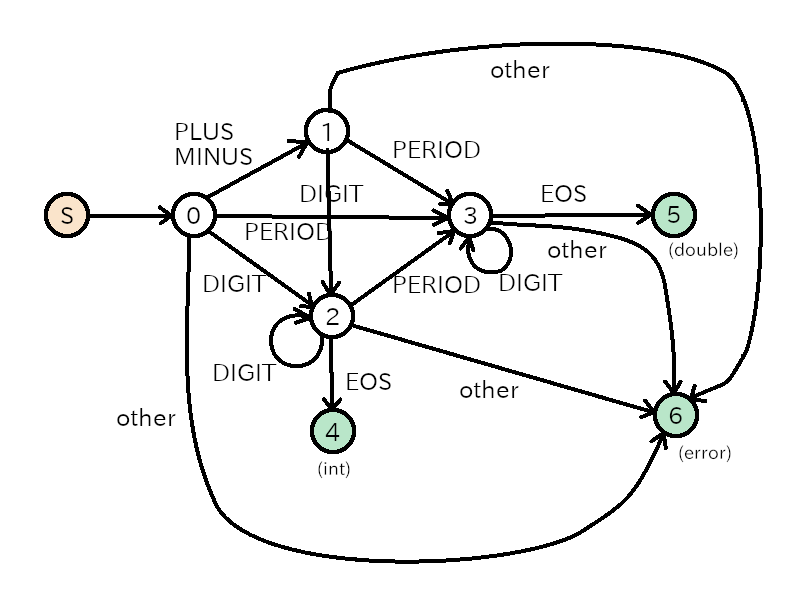
\includegraphics[width=12cm,height=9cm]{../image/state_diagram.png}
\caption{state diagram of a numeric string}
\end{figure}

The state matrix is:

\begin{longtable}[]{@{}llllll@{}}
\toprule\noalign{}
state\input & 0 & 1 & 2 & 3 & 4 \\
\midrule\noalign{}
\endhead
\bottomrule\noalign{}
\endlastfoot
0 & 1 & 2 & 3 & 6 & 6 \\
1 & 6 & 2 & 3 & 6 & 6 \\
2 & 6 & 2 & 3 & 4 & 6 \\
3 & 6 & 3 & 6 & 5 & 6 \\
\end{longtable}

This state diagram doesn't support ``1.23e5'' style double (decimal
floating point). If it is supported, the state diagram will be more
complicated. (However, it will be a good practice for your programming
skill.)

\subsection{Header file}\label{header-file}

The header file of TNumStr is \passthrough{\lstinline!tnumstr.h!}. It is
in the \passthrough{\lstinline!src/tstr!} directory.

\begin{lstlisting}[language=C, numbers=left]
#pragma once

#include <glib-object.h>
#include "tstr.h"
#include "../tnumber/tnumber.h"

#define T_TYPE_NUM_STR  (t_num_str_get_type ())
G_DECLARE_FINAL_TYPE (TNumStr, t_num_str, T, NUM_STR, TStr)

/* type of the numeric string */
enum {
  t_none,
  t_int,
  t_double
};

/* get the type of the TNumStr object */
int
t_num_str_get_string_type (TNumStr *self);

/* setter and getter */
void
t_num_str_set_from_t_number (TNumStr *self, TNumber *num);

// TNumStr can have any string, which is t_none, t_int or t_double type.
// If the type is t_none, t_num_str_get_t_number returns NULL.
// It is good idea to call t_num_str_get_string_type and check the type in advance. 

TNumber *
t_num_str_get_t_number (TNumStr *self);

/* create a new TNumStr instance */
TNumStr *
t_num_str_new_with_tnumber (TNumber *num);

TNumStr *
t_num_str_new (void);
\end{lstlisting}

\begin{itemize}
\tightlist
\item
  8: The macro \passthrough{\lstinline!G\_DECLARE\_FINAL\_TYPE!} for
  TNumStr class. It is a child class of TStr and a final type class.
\item
  11-15: These three enum data define the type of TNumStr string.

  \begin{itemize}
  \tightlist
  \item
    \passthrough{\lstinline!t\_none!}: No string is stored or the string
    isn't a numeric string.
  \item
    \passthrough{\lstinline!t\_int!}: The string expresses an integer
  \item
    \passthrough{\lstinline!t\_double!}: The string expresses an real
    number, which is double type in C language.
  \end{itemize}
\item
  18-19: The public function
  \passthrough{\lstinline!t\_num\_str\_get\_string\_type!} returns the
  type of the string TStrNum object has. The returned value is
  \passthrough{\lstinline!t\_none!}, \passthrough{\lstinline!t\_int!} or
  \passthrough{\lstinline!t\_double!}.
\item
  22-30: Setter and getter from/to a TNumber object.
\item
  33-37: Functions to create new TNumStr objects.
\end{itemize}

\subsection{C file}\label{c-file}

The C file of TNumStr is \passthrough{\lstinline!tnumstr.c!}. It is in
the \passthrough{\lstinline!src/tstr!} directory.

\begin{lstlisting}[language=C, numbers=left]
#include <stdlib.h>
#include <ctype.h>
#include "tnumstr.h"
#include "tstr.h"
#include "../tnumber/tnumber.h"
#include "../tnumber/tint.h"
#include "../tnumber/tdouble.h"

struct _TNumStr {
  TStr parent;
  int type;
};

G_DEFINE_TYPE(TNumStr, t_num_str, T_TYPE_STR)

static int
t_num_str_string_type (const char *string) {
  const char *t;
  int stat, input;
  /* state matrix */
  int m[4][5] = {
    {1, 2, 3, 6, 6},
    {6, 2, 3, 6, 6},
    {6, 2, 3, 4, 6},
    {6, 3, 6, 5, 6}
  };

  if (string == NULL)
    return t_none;
  stat = 0;
  for (t = string; ; ++t) {
    if (*t == '+' || *t == '-')
      input = 0;
    else if (isdigit (*t))
      input = 1;
    else if (*t == '.')
      input = 2;
    else if (*t == '\0')
      input = 3;
    else
      input = 4;

    stat = m[stat][input];

    if (stat >= 4 || *t == '\0')
      break;
  }
  if (stat == 4)
    return t_int;
  else if (stat == 5)
    return t_double;
  else
    return t_none;
}

/* This function overrides t_str_set_string. */
/* And it also changes the behavior of setting the "string" property. */
/* On TStr => just set the "string" property */
/* On TNumStr => set the "string" property and set the type of the string. */
static void
t_num_str_real_set_string (TStr *self, const char *s) {
  T_STR_CLASS (t_num_str_parent_class)->set_string (self, s);
  T_NUM_STR (self)->type = t_num_str_string_type(s);
}

static void
t_num_str_init (TNumStr *self) {
  self->type = t_none;
}

static void
t_num_str_class_init (TNumStrClass *class) {
  TStrClass *t_str_class = T_STR_CLASS (class);

  t_str_class->set_string = t_num_str_real_set_string;
}

int
t_num_str_get_string_type (TNumStr *self) {
  g_return_val_if_fail (T_IS_NUM_STR (self), -1);

  return self->type;
}

/* setter and getter */
void
t_num_str_set_from_t_number (TNumStr *self, TNumber *num) {
  g_return_if_fail (T_IS_NUM_STR (self));
  g_return_if_fail (T_IS_NUMBER (num));

  char *s;

  s = t_number_to_s (T_NUMBER (num));
  t_str_set_string (T_STR (self), s);
  g_free (s);
}

TNumber *
t_num_str_get_t_number (TNumStr *self) {
  g_return_val_if_fail (T_IS_NUM_STR (self), NULL);

  char *s = t_str_get_string(T_STR (self));
  TNumber *tnum;

  if (self->type == t_int)
    tnum = T_NUMBER (t_int_new_with_value (atoi (s)));
  else if (self->type == t_double)
    tnum = T_NUMBER (t_double_new_with_value (atof (s)));
  else
    tnum = NULL;
  g_free (s);
  return tnum;
}

/* create a new TNumStr instance */

TNumStr *
t_num_str_new_with_tnumber (TNumber *num) {
  g_return_val_if_fail (T_IS_NUMBER (num), NULL);

  TNumStr *numstr;

  numstr = t_num_str_new ();
  t_num_str_set_from_t_number (numstr, num);
  return numstr;
}

TNumStr *
t_num_str_new (void) {
  return T_NUM_STR (g_object_new (T_TYPE_NUM_STR, NULL));
}
\end{lstlisting}

\begin{itemize}
\tightlist
\item
  9-12: TNumStr structure has its parent ``TStr'' and int type ``type''
  members. So, TNumStr instance holds a string, which is placed in the
  parent's private area, and a type.
\item
  14: \passthrough{\lstinline!G\_DEFINE\_TYPE!} macro.
\item
  16- 54: The function
  \passthrough{\lstinline!t\_num\_str\_string\_type!} checks the given
  string and returns \passthrough{\lstinline!t\_int!},
  \passthrough{\lstinline!t\_double!} or
  \passthrough{\lstinline!t\_none!}. If the string is NULL or an
  non-numeric string, \passthrough{\lstinline!t\_none!} will be
  returned. The check algorithm is explained in the first subsection
  ``Verification of a numeric string''.
\item
  60-64: The function
  \passthrough{\lstinline!t\_num\_str\_real\_set\_string!} sets
  TNumStr's string and its type. This is a body of the class method
  pointed by \passthrough{\lstinline!set\_string!} member of the class
  structure. The class method is initialized in the class initialization
  function \passthrough{\lstinline!t\_num\_str\_class\_init!}.
\item
  66-69: The instance initialization function
  \passthrough{\lstinline!t\_num\_str\_init!} sets the type to
  \passthrough{\lstinline!t\_none!} because its parent initialization
  function set the pointer \passthrough{\lstinline!priv->string!} to
  NULL.
\item
  71-76: The class initialization function
  \passthrough{\lstinline!t\_num\_str\_class\_init!} assigns
  \passthrough{\lstinline!t\_num\_str\_real\_set\_string!} to the member
  \passthrough{\lstinline!set\_string!}. Therefore, the function
  \passthrough{\lstinline!t\_str\_set\_string!} calls
  \passthrough{\lstinline!t\_num\_str\_real\_set\_string!}, which sets
  not only the string but also the type. The function
  \passthrough{\lstinline!g\_object\_set!} also calls it and sets both
  the string and type.
\item
  78-83: The public function
  \passthrough{\lstinline!t\_num\_str\_get\_string\_type!} returns the
  type of the string.
\item
  86-113: Setter and getter. The setter sets the numeric string from a
  TNumber object. And the getter returns a TNumber object.
\item
  117-131: These two functions create TNumStr instances.
\end{itemize}

\subsection{Child class extends parent's
function.}\label{child-class-extends-parents-function.}

TNumStr is a child class of TStr, so it has all the TStr's public
funftions.

\begin{itemize}
\tightlist
\item
  \passthrough{\lstinline!TStr *t\_str\_concat (TStr *self, TStr *other)!}
\item
  \passthrough{\lstinline!void t\_str\_set\_string (TStr *self, const char *s)!}
\item
  \passthrough{\lstinline!char *t\_str\_get\_string (TStr *self)!}
\end{itemize}

When you want to set a string to a TNumStr instance, you can use
\passthrough{\lstinline!t\_str\_set\_string!} function.

\begin{lstlisting}[language=C]
TNumStr *ns = t_num_str_new ();
t_str_set_string (T_STR (ns), "123.456");
\end{lstlisting}

TNumStr extends the function
\passthrough{\lstinline!t\_str\_set\_string!} and it sets not only a
string but also the type for a TNumStr instance.

\begin{lstlisting}[language=C]
int t;
t = t_num_str_get_string_type (ns);
if (t == t_none) g_print ("t_none\n");
if (t == t_int) g_print ("t_int\n");
if (t == t_double) g_print ("t_double\n");
// => t_double appears on your display
\end{lstlisting}

TNumStr adds some public functions.

\begin{itemize}
\tightlist
\item
  \passthrough{\lstinline!int t\_num\_str\_get\_string\_type (TNumStr *self)!}
\item
  \passthrough{\lstinline!void t\_num\_str\_set\_from\_t\_number (TNumStr *self, TNumber *num)!}
\item
  \passthrough{\lstinline!TNumber *t\_num\_str\_get\_t\_number (TNumStr *self)!}
\end{itemize}

A child class extends the parent class. So, a child is more specific and
richer than the parent.

\subsection{Compilation and execution}\label{compilation-and-execution}

There are \passthrough{\lstinline!main.c!},
\passthrough{\lstinline!test1.c!} and \passthrough{\lstinline!test2.c!}
in \passthrough{\lstinline!src/tstr!} directory. Two programs
\passthrough{\lstinline!test1.c!} and \passthrough{\lstinline!test2.c!}
generates \passthrough{\lstinline!\_build/test1!} and
\passthrough{\lstinline!\_build/test2!} respectively. They test
\passthrough{\lstinline!tstr.c!} and
\passthrough{\lstinline!tnumstr.c!}. If there are errors, messages will
appear. Otherwise nothing appears.

The program \passthrough{\lstinline!main.c!} generates
\passthrough{\lstinline!\_build/tnumstr!}. It shows how TStr and TNumStr
work.

Compilation is done by usual way. First, change your current directory
to \passthrough{\lstinline!src/tstr!}.

\begin{lstlisting}
$ cd src/tstr
$ meson setup _build
$ ninja -C _build
$ _build/test1
$ _build/test2
$ _build/tnumstr
String property is set to one.
"one" and "two" is "onetwo".
123 + 456 + 789 = 1368
TNumStr => TNumber => TNumStr
123 => 123 => 123
-45 => -45 => -45
+0 => 0 => 0
123.456 => 123.456000 => 123.456000
+123.456 => 123.456000 => 123.456000
-123.456 => -123.456000 => -123.456000
.456 => 0.456000 => 0.456000
123. => 123.000000 => 123.000000
0.0 => 0.000000 => 0.000000
123.4567890123456789 => 123.456789 => 123.456789
abc => (null) => abc
(null) => (null) => (null)
\end{lstlisting}

The last part of \passthrough{\lstinline!main.c!} is conversion between
TNumStr and TNumber. There are some difference between them because of
the following two reasons.

\begin{itemize}
\tightlist
\item
  floating point is rounded. It is not an exact value when the value has
  long figures. TNumStr ``123.4567890123456789'' is converted to TNumber
  123.456789.
\item
  There are two or more string expression in floating points. TNumStr
  ``.456'' is converted to TNumber x, and x is converted to TNumStr
  ``0.456000''.
\end{itemize}

It is difficult to compare two TNumStr instances. The best way is to
compare TNumber instances converted from TNumStr.
